\section{Matching}
\subsection*{题意}
给定一个$ n+n$ 个点的二分图,求有多少种完美匹配。

\paragraph{定义:}
\begin{itemize}
\item \textit{二分图}:指顶点可以分成左右两部分,且各自内部顶点间不会有边相连的图。
\item \textit{完美匹配}:将左右顶点两两配对,但配对的顶点之间必须相邻。
\end{itemize}


\begin{center}
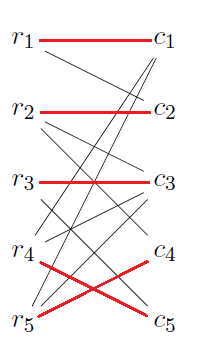
\includegraphics[width=4cm]{./Pics/Perfect Matching.png}
\end{center}
\subsection*{数据范围}
\begin{itemize}
\item $1 \leq n \leq 21$
\end{itemize}

\subsection*{题解}
这题是典型的\textbf{状态压缩}动态规划,简称状压DP,一般是指数级的复杂度。尽管复杂度很高,但比最暴力的阶乘级复杂度还是要快不少。

通常我们需要定义一个 $\texttt{mask}$ 变量来表示被选取的子集是什么。例如全集是 $\{0,1,2,3,4\}$,而选取的子集是 $\{0,2,3\}$,那么 $\texttt{mask = 10110}$,表达式为 $\texttt{(1<<0) + (1<<2) + (1<<3)}$
,其中 $\texttt{<<}$ 表示左移。

首先我们考虑暴力做法:依次考虑左边每个点和右边哪个点匹配。假设给定的图是一个二分完全图,即左右之间任意两点均可配对,那么一共有 $n!$ 种匹配方法,在 $n = 21$ 的情况下高达 $10^{19}$ 的量级,无法通过。

注意到在考虑顶点 $i$ 的搭档时,我们只关心之前的点已经占用了哪些点,而具体连接方式并不重要。举个例子,假设我们当前考虑顶点 $2$,之前选择了 $\{(0,3),(1,4) \}$
还是$\{(0,4),(1,3) \}$ 对当下的影响是相同的,即不能再使用右边的 $3$ 和 $4$。

那么我们把等价状态合并:设 $\texttt{dp}[i][\texttt{mask}]$ 表示考虑了节点 $\{0,1,\ldots,i\}$,并且使用的(右侧)点集为 $\texttt{mask}$。

转移方式很简单:对于状态$\texttt{dp}[i][\texttt{mask}]$,只需要枚举节点 $i$ 的邻居 $j$,如果 $\texttt{mask}$ 包含 $j$,方案数等于所有 $\texttt{dp}[i-1][\texttt{mask - (1<<j)}]$ 之和。

更进一步地,因为$\{0,1,\ldots,i\}$一共有 $i+1$ 个节点,所以仅当 $\texttt{mask}$中 $\texttt{1}$ 的数量等于$i + 1$时状态才有意义。于是我们只需要保留 $\texttt{mask}$ 这一维,另一维 $i$ 可以直接设为$\texttt{\_\_builtin\_popcount(mask)-1} $,其中 $\texttt{\_\_builtin\_popcount}$ 表示二进制下 $\texttt{1}$ 的数量。

不难发现,$\texttt{mask}$ 的转移一定是从小的数字转移到大的数字,如 $\texttt{1000} \rightarrow \texttt{1001}$,所以我们只需要从小到大枚举 $\texttt{mask}$ 即可。






\subsection*{核心代码}
\inputminted[linenos,autogobble]{cpp}{./Code/O.cpp}
\newpage